\documentclass{article}

\usepackage{kotex}
\usepackage{graphicx}
\usepackage[affil-it]{authblk}
\usepackage{mathtools}
\usepackage{amssymb}
\usepackage{amsthm}
\usepackage{geometry}
\usepackage{fancyhdr}
\usepackage{braket}
\usepackage{cite}
\usepackage{cancel}
\usepackage{subcaption}
\usepackage{enumitem}
\usepackage{color}
\usepackage{chemformula}
\usepackage{physics}
\usepackage{hyperref}

\newcommand{\vp}{\varphi}
\newcommand{\ve}{\varepsilon}

\newtheorem{theorem}{Theorem}
\newtheorem{definition}[theorem]{Definition}
\newtheorem{example}[theorem]{Example}
\newtheorem{lemma}[theorem]{Lemma}
\newtheorem{axiom}[theorem]{Axiom}
\newtheorem{remark}[theorem]{Remark}
\newtheorem{problem}[theorem]{Problem}
\newtheorem{exercise}[theorem]{Exercise}

\counterwithin{equation}{section}
\counterwithin{theorem}{section}


\geometry{a4paper,left=2cm,right=2cm,top=2.4cm,bottom=2.4cm}

\linespread{1.3}

\title{\textsf{Boltzmann Statics}}
\author[1]{Written by Eun Taek Kang\thanks{email: etkang03@gmail.com}}
\affil[1]{Department of Physics, Sogang University, Seoul 04107, Korea}

\date{Summer 2025, Sogang University}

\begin{document}

\pagestyle{fancy}
    %... then configure it.
    \fancyhf{}
    % Set the header and footer for Even
    % pages but omit the zone (L, C or R)
    \fancyhead[R]{\textsf{Prof.\ Hyeonjun Baek}}
    \fancyhead[L]{\textsc{Thermal Physics}}
    \fancyfoot[C]{\thepage}
    \fancyfoot[L]{\textbf{Sogang University}}
    \fancyfoot[R]{\textit{Department of Physics}}

\maketitle

\begin{abstract}
    백현준 교수님께서 2025년 1학기에 진행하는 열역학 기말고사 대비를 위해 만든 Note입니다. 이 문서는 Daniel V. Schroeder 저 An Introduction to Thermal Physics의 Chapter 6. Boltzmann statistics를 다루고 있습니다.
\end{abstract}

\newpage

\section{The Boltzmann Factor}

\textbf{Introduction}

\begin{figure}[h]
    \centering
    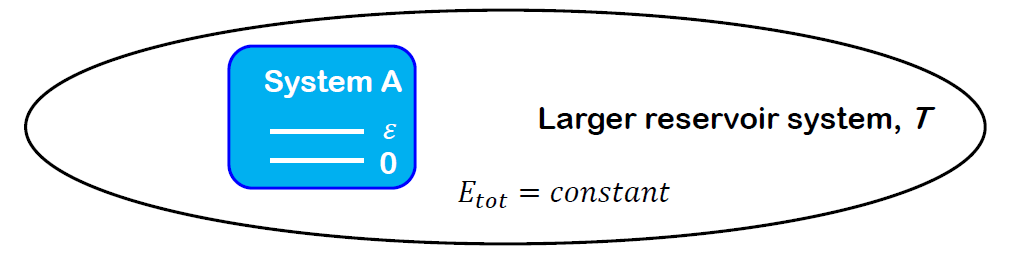
\includegraphics[width=0.65\linewidth]{images/fig1_1.png}
\end{figure}

먼저, 온도가 $T$고, 에너지는 0 또는 $\ve$, 에너지의 총합($E_{tot}$)은 상수인 계 $A$를 가정하자. 엔트로피는 다음과 같다.
\begin{equation}\label{eq:1-1}
    S(E) = k \ln \Omega (E)
\end{equation}
따라서, 각 에너지에 대한 number of states는 이렇다.
\begin{align}
    (\text{State of $\ve$}) &= 1 \times \Omega(E_{tot} - \ve) = \exp[S(E_{tot} - \ve) / k]\\
    (\text{State of $0$}) &= 1 \times \Omega(E_{tot}) = \exp [S(E_{tot})/k]
\end{align}

\noindent
여기서, $S(E_{tot} - \ve)$는 다음과 같이 근사할 수 있다.
\begin{equation}
    S(E_{tot} - \ve) = S(E_{tot}) - \ve \left( \frac{\partial S}{\partial E} \right)_{E=E_{tot}} + \cdots
\end{equation}
이 두 인자들을 나눠주고, $(\partial S/ \partial E) = 1/T$임을 이용해 정리해주면 다음과 같다.
\begin{equation}
    \frac{\Omega (E_{tot} - \ve)}{\Omega (E_{tot})} = e^{-\ve / kT}
\end{equation}

\noindent
\textbf{The partition function}
\begin{equation}
    Z = \sum_s e^{-E(s)/kT} \quad \text{(Sum of all Boltzmann factor)}
\end{equation}
이때, $s$라는 state가 나올 확률을 $\mathcal{P}(s)$라고 하자. $\mathcal{P}(s)$는 다음과 같다.
\begin{equation}
    \mathcal{P}(s) = \frac{1}{Z} e^{-E(s)/kT} = \frac{1}{Z} e^{-\beta E(s)} \quad (\beta = 1/kT)
\end{equation}
우리는 이 $\beta$에 대한 notation을 조금 더 많이 활용하기로 할 것이다.

\section{Average Values}

앞서 봤던 확률함수로 에너지의 평균값을 구하면 다음과 같다.
\begin{equation}
    \overline{E} = \sum_s E(s) \mathcal{P}(s) = \frac{1}{Z} \sum_s E(s) e^{-E(s)/kT}
\end{equation}
어렵게 생각할 필요 없이 고등학교에서 배운 확률과 통계를 잘 생각하면 obvious하다! 이를 any quantity $X(s)$에 대해 일반화 하면 다음과 같다.
\begin{equation}
    \overline{X} = \frac{1}{Z} \sum_s X(s) e^{-E(s)/kT}
\end{equation}

\newpage

\noindent
\textbf{Micro-caonical ensemble vs Canonical ensemble}

\begin{figure}[h]
    \centering
    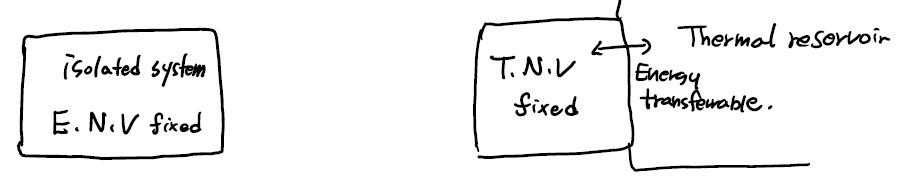
\includegraphics[width=0.8\linewidth]{images/fig2_1.png}
\end{figure}
In \textcolor{blue}{micro-canonical} ensemble, $\Omega (E,N,V)$는 multiplicity이다. 이때, 모든 accessible state(앙상블의 원소)는 다 확률이 동일하다.

In \textcolor{blue}{canonical} ensemble, 모든 state들의 확률들은 Boltzmann factor $e^{-E/kT}$에 의해 나눠진다. 

\vspace{3mm}\noindent
\textbf{Use relation for Average energy}

평균 에너지에 대해서 다음과 같은 관계가 성립한다.
\begin{equation}
    \overline{E} = -\frac{1}{Z} \frac{\partial Z}{\partial \beta} = -\frac{\partial}{\partial \beta} \ln Z
\end{equation}

\begin{proof}
    $Z = \sum_{s} e^{-\beta E(s)}$에서 출발하자.
    \begin{equation*}
        \frac{\partial Z}{\partial \beta} = \sum_s (-E(s)) e^{-\beta E(s)} \quad \Rightarrow \quad \overline{E} = \frac{1}{Z} \sum_s E(s) e^{-\beta E(s)} = -\frac{1}{Z} \frac{\partial Z}{\partial \beta}
    \end{equation*}
\end{proof}

\noindent
\textbf{Paramagnetism}

이제, Boltzmann factor를 2개의 state를 가진 paramagnet에 적용해 볼 것이다. 강자성체가 가지는 ideal한 2가지 state는 다음과 같다.
\begin{equation*}
    \begin{cases}
        \uparrow \ : E = -\mu B \\
        \downarrow \ : E = + \mu B
    \end{cases}
\end{equation*}
여기서, partition function을 계산해주면,
\begin{equation}
    Z  = \sum_s e^{-\beta E(s)} = e^{\beta \mu B} + e^{-\beta \mu B} = 2\cosh (\beta \mu B)
\end{equation}
이어서, 평균 에너지를 계산해주면,
\begin{equation}
    \overline{E} = \frac{1}{Z} \sum_s E(s) e^{-\beta E(s)} = \frac{-\mu B [e^{\beta \mu B} - e^{-\beta \mu B}]}{2\cosh (\beta \mu B)} = -\mu B \tanh (\beta \mu B)
\end{equation}
추가적으로, $N$ dipoles에 대한 collection(전체 에너지)는 dipole의 개수 $N$에 평균 에너지 $\overline{E}$를 곱하여 얻는다.
\begin{equation}
    U = N\overline{E} = -N \mu B \tanh (\beta \mu B)
\end{equation}

\noindent
\textbf{Note:} 앞서 Chapter 3에서 얻은 결과들을 다시 보자.
\begin{equation}
    S/k = \ln Omega = \ln \frac{N!}{N_\uparrow ! N_\downarrow !}, \quad U = \mu B (N - 2N_\uparrow)
\end{equation}
여기서 다음 관계식을 이용해 더 정리해주면, 다음과 같다.
\begin{equation}
    \frac{1}{T} = \left( \frac{\partial S}{\partial U} \right)_{N, B} \quad \Rightarrow \quad U = U(T)
\end{equation}
두 앙상블은 같은 결과를 주나, 보통 canonical 앙상블에서 가장 확률이 큰 에너지 $E^*$에 대해 볼츠만 팩터가 좀 더 크다. 따라서 두 앙상블이 같은 것은 아니다. (Problem 6.18을 참고하라!)

\newpage

\noindent
\textbf{Rotation of diatomic molecules}

회전 운동 에너지는 고전적으로 다음과 같이 계산했다.
\begin{equation}
    E_{rot} = \frac{L_x ^2}{2I_x} + \frac{L_y ^2}{2I_y}
\end{equation}
양자역학적으론 다음과 같이 계산했다.
\begin{equation}
    E(j) = j(j+1)\epsilon \quad (\text{with degeneracy $2j+1$})
\end{equation}
이 떄, 회전 운동 에너지에 대한 partition function은 다음과 같다.
\begin{equation}
    Z_{rot} = \sum_{j=0}^{\infty} (2j+1) e^{-j(j+1)\epsilon/kT}
\end{equation}

\begin{figure}[h]
    \centering
    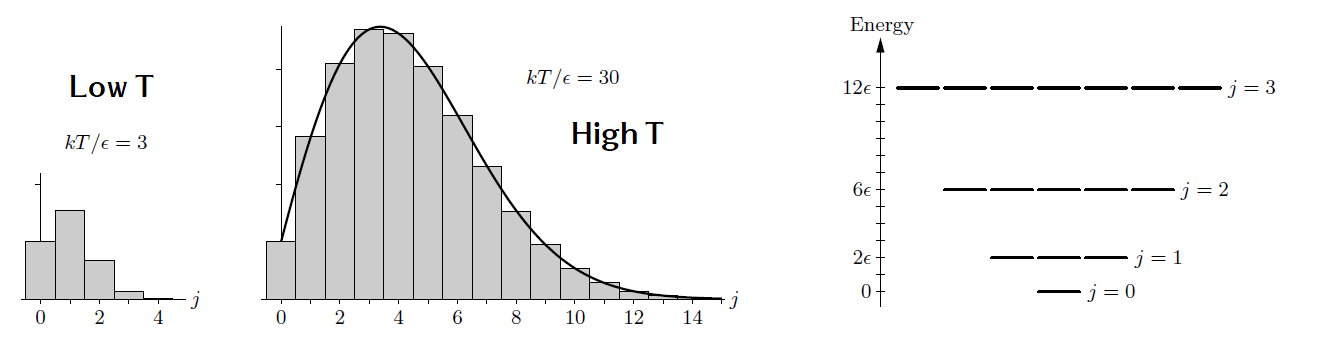
\includegraphics[width=1\linewidth]{images/fig2_2.png}
\end{figure}

$kT \gg \epsilon$(열에너지가 준위 간 에너지보다 훨씬 클 때)에는, 분배 함수에 크게 기여하는 항들이 매우 많아진다. 따라서 partition function은 다음처럼 근사할 수 있다.
\begin{equation}
    Z_{tot} \approx \int_0^\infty (2j+1) e^{-j(j+1) \epsilon / kT} dj
\end{equation}
여기서, 지수함수의 분자를 변수 치환해준다. $x \equiv j(j+1)\epsilon / kT$이면, $dx = (2j+1)\epsilon /kT dj$이므로,
\begin{equation}
    \int_0^\infty \frac{kt}{\epsilon} e^{-x} dx = \frac{kT}{\epsilon} [-e^{-x}]_0^\infty = \frac{kT}{\epsilon}
\end{equation}

한 술 더 떠서, $\overline{E} = -(\partial/\partial \beta) \ln Z$를 이용해서 평균 회전에너지를 구하면 다음과 같다.
\begin{equation}
    \overline{E_{tot}} = -\frac{\partial}{\partial \beta} \ln (1/\beta \epsilon) = \frac{1}{\beta} = kT \quad (\text{when }kT \gg \epsilon)
\end{equation}
뭔가 나중에 나올 equipartition theorem $\overline{E} = f \cdot kT$이 예측한 의미를 정확히 보여주는 꼴인 듯 하다..

\begin{figure}[h]
    \centering
    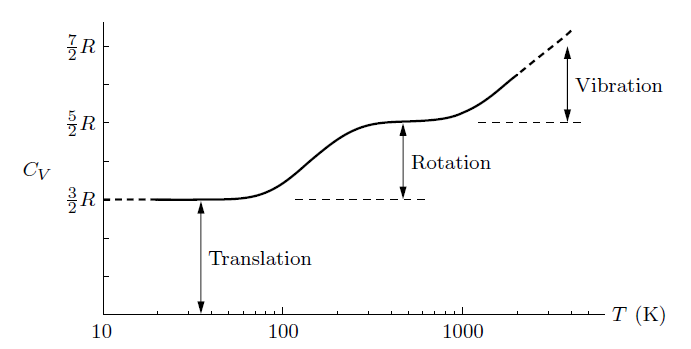
\includegraphics[width=0.65\linewidth]{images/fig2_3.png}
\end{figure}

\newpage

앞의 열용량 그래프에서, 이원자 분자가 구분 가능한 원자로 이루어진 경우 (예: CO), 이전의 결과는 맞다. 그러나, 동일한 원자로 구성된 분자들의 경우, 구별 불가능성을 고려해야 한다.

가령 \ch{O2}같은 경우, 분자를 $180^\circ$만큼 회전시켜도 위상적으로 동일한 상태이다. 이는 곧 그 분자는 \textbf{가능한 상태 수가 원래보다 절반}임을 나타낸다.

이때, 회전 에너지의 분배함수는
\begin{equation}
    Z_{rot} = \frac{kT}{2 \epsilon} \quad (kT \gg \epsilon)
\end{equation}
이 되어 기존의 절반 값이 되지만, 평균 에너지는 Z에 상수배를 해도 변화가 없음을 다음과 같이 알 수 있다.
\begin{equation}
    \overline{E_{rot}} = -\frac{1}{Z} \frac{\partial Z}{\partial B}
\end{equation}

\section{The Equipartition Theorem}

\textbf{Equipartition theorem}

\begin{theorem}[Equipartition theorem]
    System whose energy is in the form of quadratic degrees of freedom
    \begin{equation}
        E = \sum_i^f c_i q_i^2 \quad \Rightarrow \quad \overline{E} = \frac{f}{2} \cdot kT
    \end{equation}
    when $f$ is degrees of freedom, $q$ is coordinate, momentum variable.
\end{theorem}

앞에서도 봤겠지만, 에너지의 표현이 이차항에 비례할 경우, 평균 에너지는 DOF에만 의존한다는 정리다. 예를 들어 보자.
\begin{align}
    E_{trans} = \frac{p_x^2}{2m} + \frac{p_y^2}{2m} + \frac{p_z^2}{2m} \quad &\Rightarrow \quad \overline{E}_{trans} = \frac32 kT\\
    E_{vib} = \frac{p_x^2}{2m} + \frac12 kx^2 \quad &\Rightarrow \quad \overline{E}_{vib} = \frac22 kT\\
    E_{rot} = \frac{L_x^2}{2L_x} + \frac{L_y^2}{2L_y} \quad &\Rightarrow \quad \overline{E}_{rot} = kT
\end{align}

\begin{proof}
    Boltzmann factor를 이용해 equipartition theorem을 증명해보자. Suppose an system with $E = cq^2$. 이 때, 분배 함수는 다음과 같다. ($\Delta q$가 아주 작다고 가정했당)
    \begin{equation}
        Z = \sum_q e^{-\beta cq^2 } = \frac{1}{\Delta q} \sum_q e^{-\beta c q^2} \Delta Q \approx \frac{1}{\Delta q} \int_{-\infty}^\infty e^{\beta c q^2} dq
    \end{equation}
    분자를 잘 치환하자. $x \equiv \sqrt{\beta c} q$이므로, $dx = \sqrt{\beta c} dq$임을 이용해주면,
    \begin{equation}
        \frac{1}{\Delta q} \int_{-\infty}^\infty e^{\beta c q^2} dq = \frac{1}{\Delta q} \frac{1}{\sqrt{\beta c}} \int_{-\infty}^{\infty} e^{-x^2} dx = \frac{1}{\Delta q} \frac{1}{\sqrt{\beta c}} \sqrt{\pi} = C \beta^{-1/2}
    \end{equation}
    여기서 $C$는 상수이다. $Z = C\beta^{-1/2}$임을 이용해 $\overline{E}$를 구하자.
    \begin{equation}
        \overline{E} = - \frac{\partial}{\partial \beta} \ln Z = -\frac{1}{Z} \frac{\partial Z}{\partial \beta} = -\frac{1}{C\beta^{-1/2}} \frac{\partial}{\partial \beta} C\beta^{-1/2} = \frac{1}{2\beta} = \frac{1}{2} kT
    \end{equation}
\end{proof}

\noindent
\textbf{Note}: 등분배 법칙(The equipartition theorem)은 무조건 고온(high-temperature limit)에서 성립한다. 추가적으로, 분포에는 많은 state들이 기여하기에, 그들의 간격은 크게 중요치 않다.

\newpage

\section{The Maxwell Speed Distribution}

\noindent
\textbf{Distribution of gas molecule speed at temperature $T$}

\begin{figure}[h]
    \centering
    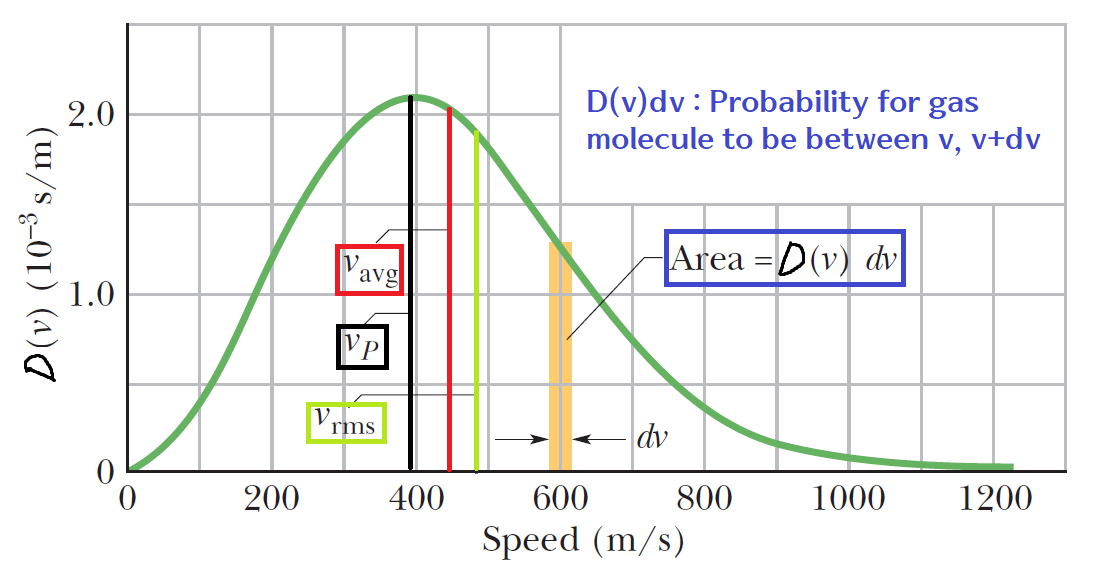
\includegraphics[width=0.75\linewidth]{images/fig4_1.png}
\end{figure}

\noindent
$v_P$는 most probable speed, $v_{\text{avg}}$는 average speed, $v_{\text{rms}}$는 root-mean-square speed이다.
\begin{equation}
    \boxed{v_P = \sqrt{\frac{2RT}{M}} \ \ (\text{most probable speed})} \ \ <  \ \ \boxed{v_{\text{avg}} = \sqrt{\frac{8RT}{\pi M}}} \ \ < \ \ \boxed{v_{\text{rms}} = \sqrt{\frac{3RT}{M}} \ \ (\text{rms speed})}
\end{equation}

다음과 같은 함수의 그래프를 생각하자.

\begin{figure}[h]
    \centering
    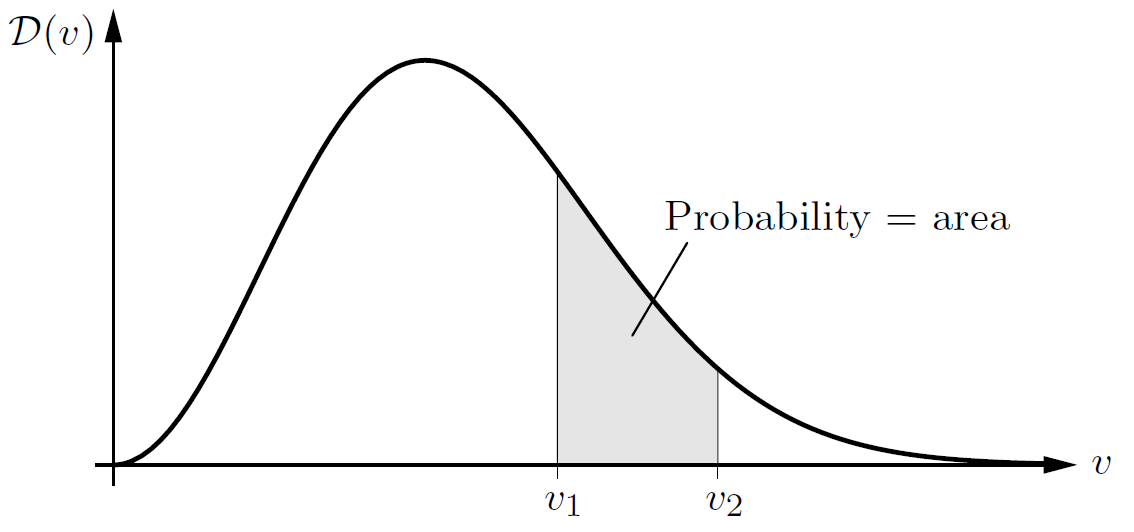
\includegraphics[width=0.6\linewidth]{images/fig4_2.png}
\end{figure}

$\mathcal{D}(v)$를 우리는 분포 함수(Distribution function)이라고 한다. 익숙한 대상이다. 우리는 이걸 속력 분포 함수로 나타내고 싶은 것이다.

속력 분포 함수 $\mathcal{D}(v)$는 두 항에 비례한다. \textbf{1.} 분자가 속력을 가질 확률 $e^{-mv^2/2kT}$, \textbf{2.} 속력 $v$일 때, 그 속력을 가지는 벡터들의 수 (겉넓이) $4\pi v^2$.
\begin{equation}
    \mathcal{D}(v) = C \cdot 4\pi v^2 e^{-mv^2/2kT}
\end{equation}
변수를 바꾼 다음 정규화 해줄건데, 지수함수가 가우시안 적분이 되도록 변수를 이렇게 잡는다.
\begin{equation}
    x \equiv \sqrt{\frac{m}{2kT}} v \quad \Rightarrow \quad dx = \sqrt{\frac{m}{2kT}} dv
\end{equation}
정규화 해주자.
\begin{align} \nonumber
    1 &= \int_0^\infty C \cdot 4\pi v^2 e^{-mv^2/2kT} dv = \int_0^\infty C \cdot 4\pi x^2 \left( \frac{2kT}{m} \right)^{3/2} e^{-x^2} dx\\
    &= 4\pi C \left( \frac{2kT}{m} \right)^{3/2} \int_0^\infty x^2 e^{-x^2} dx
    = 4\pi C \left( \frac{2kT}{m} \right)^{3/2} \frac{\sqrt{\pi}}{4} = C \left( \frac{2\pi kT}{m} \right)^{3/2}
\end{align}

\newpage

$C = (m/2\pi kT)^{3/2}$이므로, 분포 함수 $\mathcal{D}(v)$의 식은 다음과 같다.
\begin{equation}\label{mbdis}
    \boxed{\mathcal{D}(v) = \left( \frac{m}{2\pi k T} \right)^{3/2} 4\pi v^2 \cdot e^{-mv^2/2kT}}
\end{equation}
(\ref{mbdis})와 같은 분포를 이상기체 분자의 속도에 대한 \textbf{Maxwell-Boltzmann Distribution}이라구 한다!! 

\begin{figure}[h]
    \centering
    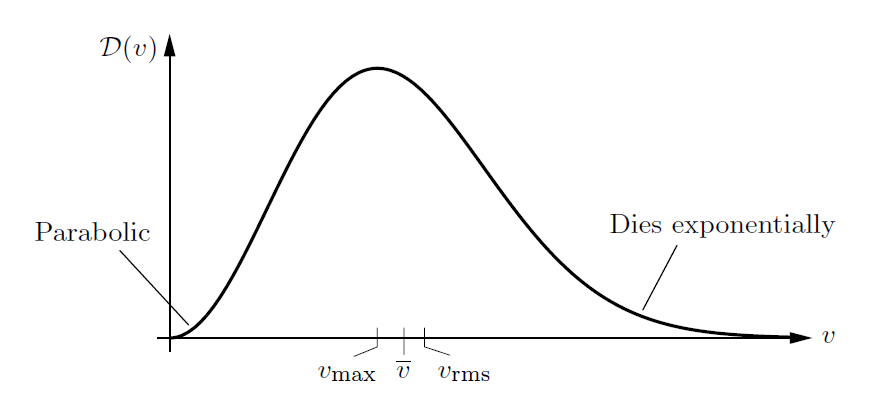
\includegraphics[width=0.65\linewidth]{images/fig4_3.png}
    \caption{Maxwell-Boltzmann 분포의 그래프}
\end{figure}

이 분포를 줄여서 Maxwell 분포라고도 부른다. 이 분포에서 나오는 3가지 속도들을 계산해보자!!\footnote{적분 계산 중 모든 $v$는 이전처럼 지수를 $-x^2$ 꼴이 나오도록 치환한다.}

\vspace{3mm} \noindent
\textbf{Most probable speed $v_{\text{max}}$}

가장 많이 나타나는 속도는 분포의 극점을 계산해주면 된다.
\begin{align} \nonumber
    \frac{d\mathcal{D} (v)}{dv} &= \cancel{\left( \frac{m}{2\pi k T} \right)^{3/2}} \left[ 2v \cdot e^{-mv^2/2kT} - v^2 \cdot \frac{mv}{kT} e^{-mv^2/2kT} \right] = 0\\
    &\Rightarrow \quad v^2 \frac{m}{kT} = 2 \quad \Rightarrow \quad \boxed{v_{\text{max}} = \sqrt{\frac{2kT}{m}}}
\end{align}

\noindent
\textbf{Average speed $\overline{v}$}

어떤 분포의 평균은 모든 지점에서의 확률과 변량의 곱을 합해서 구한다.

\begin{align} \nonumber
    \overline{v} = \int_0^\infty v \mathcal{D}(v) dv &= \left( \frac{m}{2\pi k T} \right)^{3/2} \cdot 4\pi \int_0^\infty v^3 e^{-mv^2/2kT} dv\\ \nonumber
    &= \left( \frac{m}{2\pi k T} \right)^{3/2} \cdot 4\pi \cdot \left( \frac{2kT}{m} \right)^2 \int_0^\infty x^3 e^{-x^2}dx\\
    &= \left( \frac{2kT}{m} \right)^{1/2} \cdot \pi^{-1/2} \cdot 4 \cdot \frac12 = \left( \frac{8kT}{m\pi} \right)^{1/2} \ \ \Rightarrow \ \ \boxed{\overline{v} = \sqrt{\frac{8kT}{m\pi}}}
\end{align}

\noindent
\textbf{Root-mean-square speed $v_{\text{rms}}$}

어떤 분포에서 rms point는 모든 지점에서의 확률과 (변량)$^2$의 곱을 합해서 그 제곱근으로 구한다.

\begin{align} \nonumber
    v_{\text{rms}}^2 = \int_0^\infty v^2 \mathcal{D}(v)dv &= \int_{0}^{\infty} \left( \frac{m}{2\pi k T} \right)^{3/2}  \cdot 4\pi \cdot v^4 e^{-mv^2/2kT}dv \\ \nonumber
    &= \left( \frac{m}{2\pi k T} \right)^{3/2} \cdot 4\pi \cdot \left( \frac{2kT}{m} \right)^{5/2} \int_0^\infty x^4 e^{-x^2} dx\\
    &= \left( \frac{m}{2\pi k T} \right)^{3/2} \cdot 4\pi \cdot \left( \frac{2kT}{m} \right)^{5/2} \cdot \frac{3\sqrt{\pi}}{8} = \frac{3kT}{m} \ \ \Rightarrow \ \ \boxed{v_{\text{rms}} = \sqrt{\frac{3kT}{m}}}
\end{align}

\newpage

\section{Partition function and free energy}

\textbf{Intuitive guess}

\begin{figure}[h]
    \centering
    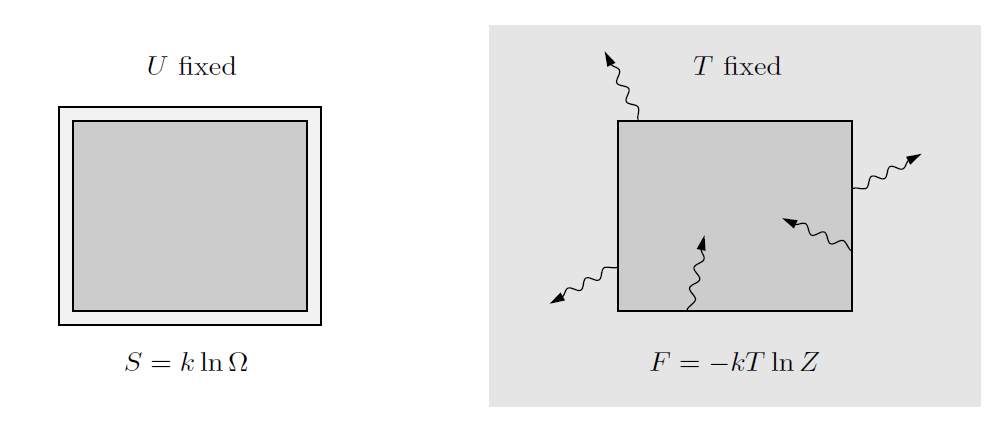
\includegraphics[width=0.7\linewidth]{images/fig5_1.png}
\end{figure}

\begin{itemize}
    \item $U$가 고정된 microcanonical ensemble에선 엔트로피 $S$가 증가하는 경향을 보인다.
    $$\frac{S}{k} = \ln \Omega \quad \text{(dimensionless)}$$
    \item $T$가 고정된 canonical ensemble에선 Helmholtz free energy $F$가 감소하는 경향을 보인다.
    $$-\frac{F}{kT} = \ln Z \quad \Rightarrow \quad F = -kT\ln Z$$
\end{itemize}

\begin{proof}
    Recall that $U = \dfrac{\partial}{\partial \beta } \ln Z$ and $\dfrac{\partial \beta}{\partial T} = -\dfrac{1}{kT^2} = -k\beta^2$. 앞서 5장에서 배운 관계들도 보자.
    \begin{equation}
        F \equiv U - TS, \quad - \left( \frac{\partial F}{\partial T} \right)_{V,N} = S
    \end{equation}
    앞서 배운 Helmholtz Free Energy의 정의와, 그 편미분의 관계를 통해 $U$를 표현해주자. 
    \begin{align} \nonumber
        U = F + TS &= F - T \left( \frac{\partial F}{\partial T} \right)_{V,N} = F - \frac{1}{k \beta} \frac{\partial F}{\partial \beta} \cdot \frac{\partial \beta}{\partial T}\\
        &= F + \beta \frac{\partial F}{\partial \beta} = \frac{\partial}{\partial \beta} [\beta F]
    \end{align}
    $U$에 대한 관계식 2개를 비교하면 다음을 얻는다.
    \begin{equation}
        \beta F = \ln Z + C \quad (C\text{ is constant})
    \end{equation}
    $T \rightarrow 0$을 고려해서 상수를 결정하자. $F$는 바닥상태 에너지 $U_0$이 될거고, 분배함수 $Z$는 다음과 같다.
    \begin{equation}
        Z = \sum e^{-U/kT} = e^{-U_0 / kT} \ \ \rightarrow \ \ \ln Z = \frac{1}{kT} U_0 = \beta F
    \end{equation}
    따라서 상수 $C$는 0으로 결정된다. ($C=0$)
\end{proof}

\vspace{2mm}
\color{red}
우리가 방금 얻었던 $F=-kT\ln Z$의 여러가지 편미분을 통해 엔트로피, 압력, 화학 퍼텐셜을 구하는 공식들이 유용하니 잘 봐두자. When $F = U - TS \ \ \Rightarrow \ \ dF = dU - TdS - SdT$, \color{black}
\begin{equation}
    \boxed{ \color{red} S = -\left( \frac{\partial F}{\partial T} \right)_{V, N}, \quad P = -\left( \frac{\partial F}{\partial V} \right)_{T, N}, \quad \mu = +\left( \frac{\partial F}{\partial N} \right)_{T, V}} \color{black}
\end{equation}

\newpage
\color{black}
\section{Partition Functions for Composite System}

\textbf{For two particle system}

이번엔 복합계(composite system)을 다룰 것이다. 먼저 두 입자로 이루어진 계를 고려해보자. 둘이 서로 상호작용 없으면 $E_{tot} = E_1 + E_2$일 것이다. 복합계의 상태들을 $s$라 하자. 서로 독립적인 입자이므로 Summation의 분리가 가능할거다.
\begin{align} \nonumber
    Z_{\text{tot}} &= \sum_s e^{-\beta [E_1(s) + E_2(s)]} = \sum_s e^{-\beta E_1 (s)} e^{-\beta E_2 (s)}\\
    &= \sum_{s_1} e^{-\beta E_1 (s_1)} \cdot \sum_{s_2} e^{-\beta E_2 (s_2)} = Z_1 \cdot Z_2
\end{align}
이를 통해서 $N$개의 입자에 대해 일반화 해주면 전체 분배함수는 다음과 같다.
\begin{equation}
    Z_{\text{tot}} = Z_1 Z_2 Z_3 \cdots Z_N = \prod_{n=1}^N Z_n
\end{equation}


\noindent
\textbf{For non-interacting \& indistinguishable particles}

만약, 두 입자가 서로 상호작용하지 않으나, \underline{두 입자가 서로 구별되지 않는다}면 어떨까?  

\begin{figure}[h]
    \centering
    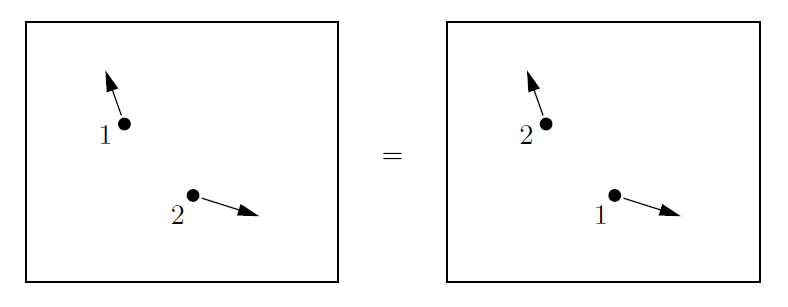
\includegraphics[width=0.7\linewidth]{images/fig6_1.png}
\end{figure}

그림과 같이 단순히 생각하면 같은 상태를 2번씩 중복해서 세준다 볼 수 있다. 따라서, 전체 분배함수는 이렇다.
\begin{equation}
    Z_{\text{tot}} = \frac12 Z_1 \cdot Z_2
\end{equation}
이것도 사실 완벽한 공식은 아니지만 합당하다곤 할 수 있는 정도다. $N$개의 입자에 대해 일반화하자.
\begin{equation}
    Z_{\text{tot}} = \frac{1}{N!} Z_1 Z_2 \cdots Z_N = \frac{1}{N!} Z_1^N
\end{equation}

\newpage

\section{Ideal Gas Revisited}

\textbf{The partial function}

6.6에서 봤던 N개 입자계의 분배함수는 다음과 같다.
\begin{equation}
	Z_N = \frac{1}{N!} Z_1^N
\end{equation}
$Z_1$도 한 번 써보자.
\begin{equation}\label{eq:7-2}
	Z_1 = \sum_s e^{-E(s)/kT} = \sum_s e^{-E_{\text{trans}}/kT} \sum_s e^{-E_{\text{inter}}/kT}  = Z_{\text{trans}} Z_{\text{inter}}
\end{equation}
병진 운동이랑 interal(회전, 진동같은거)는 둘이 독립적이라 $Z$도 아주 잘 쪼개진다. 보통 interal state는 고온에서 들뜬상태이다. 따라서, \textbf{병진의 분배함수}에 초점 맞춰볼것임. \underline{한 변의 길이가 $L$인 정육면체 box}를 가정해보자!

\begin{figure}[h]
    \centering
    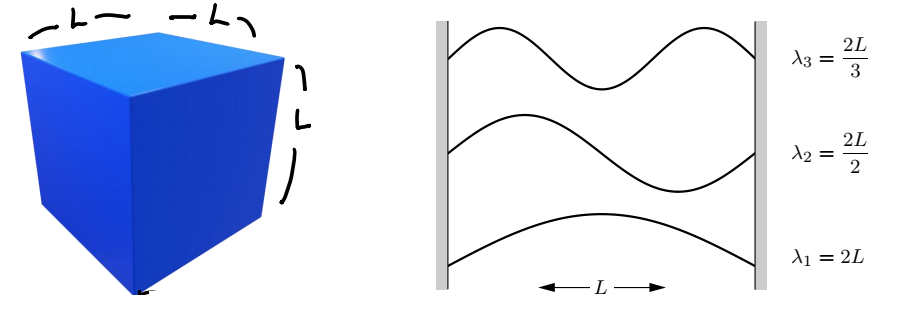
\includegraphics[width=0.7\linewidth]{images/fig7_1.png}
\end{figure}

\noindent
\textbf{In 1-dimension}

파동함수의 꼴은 다음과 같다. (당연함, 양자1을 했으면 obvious)
\begin{equation}
	\psi(x) = \sqrt{\frac{2}{L}} \sin \left( \frac{n\pi x}{L} \right), \quad k = \frac{n \pi}{L} \quad (\text{Boundary condition})
\end{equation}
그러면, 에너지는 이렇구 ($8mL$ 버전은 고등학교때도 잘 배웠지) 여기서 $k$는 파수다.
\begin{equation}
	E_n = \frac{\hbar^2 k^2}{2m} = \frac{\hbar^2 \pi^2}{2mL^2} \cdot n^2 = \frac{h^2}{8mL^2} \cdot n^2
\end{equation}
분배 함수를 구해보자. (밑에 $k$는 볼츠만 상수니까 위에 $k$는 앵간하면 죽여주자.)
\begin{equation}
	Z_{1d} =  \sum_s e^{- E_n / kT} = \int_0^\infty \exp \left[ -\frac{\hbar^2 \pi^2}{2mL^2} \cdot \frac{n^2}{kT} \right] dn = \frac{\sqrt{\pi}}{2} \times \sqrt{\frac{2mL^2 kT}{\hbar^2 \pi^2}} = L \sqrt{\frac{mkT}{2\pi \hbar^2}} = \frac{L}{l_Q}
\end{equation}
이제 뭐 가우시안은 치환 없이 잘 해야하고.. $l_Q$는 양자 길이(quantum length)인데, 다음과 같이 정의한다.
\begin{equation}
\color{blue} l_Q \equiv \sqrt{\frac{2\pi \hbar^2}{mkT}} \color{black}
\end{equation}
여하튼, 우리는 드브로이의 물질파 파장 공식을 알고 있다. $\lambda = h / E$ (일반물리 수준) 이걸 $kT$와 함께 써보자.
\begin{equation}
    E = \frac{1}{2}kT = \frac{\hbar^2}{2m} \left( \frac{2\pi}{\lambda} \right)^2  \quad \Rightarrow \quad \lambda = \sqrt{2\pi} \cdot \sqrt{\frac{2\pi \hbar^2}{mkT}}
\end{equation}
차원 분석을 잘 해보면 $l_Q$와 $\lambda$는 두 물리량의 차원이 같다. 따라서 뭉그러뜨려서 이럴 수 있다.
\begin{equation}
    \lambda \sim l_Q
\end{equation}

\newpage

\noindent
\textbf{In 3-dimension}

이제, 3차원 상황에서 알아볼건데, 3차원이면 병진, 회전 다 일어날거거든.. 병진 에너지는 다음과 같았다.
\begin{equation}
    E_{\text{tr}} = \frac{p_x^2}{2m} + \frac{p_y^2}{2m} + \frac{p_z^2}{2m}
\end{equation}
이를 통해서 분배함수를 써주면 다음과 같다. $x, y, z$축의 운동은 각각 독립적이므로
\begin{equation}
    Z_{tr} = \sum_{n_x,n_y, n_z}\exp \left[ -\frac{\hbar^2 \pi^2}{2mL^2} \frac{n_x^2}{kT} -\frac{\hbar^2 \pi^2}{2mL^2} \frac{n_y^2}{kT} -\frac{\hbar^2 \pi^2}{2mL^2} \frac{n_z^2}{kT} \right] = \frac{L_x L_y L_z}{(l_Q)^3} = \frac{V}{v_Q}
\end{equation}
여기서 $v_Q$는 quantum volume이다.
\begin{equation}
    v_Q \equiv \left( \frac{2\pi \hbar^2}{mkT} \right)^{3/2}
\end{equation}
따라서 (\ref{eq:7-2})와 결합하면 $Z_1$은 다음과 같다.
\begin{equation}
    Z_1 = \frac{V}{v_Q} Z_{\text{int}}
\end{equation}
이제, 이걸 $N$개의 분자들에 대하여 분배 함수를 작성하면
\begin{equation}
    Z = \frac{1}{N!} \left( \frac{VZ_{\text{int}}}{v_Q} \right)^N
\end{equation}
여기에 로그를 취해줄건데, $N!$에 대해선 스털링 근사를 좀 조져주면 된다.
\begin{equation}
    \ln Z = N[\ln V + \ln Z_{\text{int}}-\ln N - \ln v_Q + 1]
\end{equation}
\textbf{Prediction}

\noindent
이제, 이런 분배함수들을 통하여 우린 이상기체(ideal gas)의 열역학적 여러 properties를 계산할 수 있당.
\begin{enumerate}
    \item[\textbf{(1)}] \textbf{에너지}: $U = -\dfrac{\partial }{\partial \beta} \ln Z  = -N -\dfrac{\partial }{\partial \beta} \ln Z_{\text{int}} + N\dfrac{1}{v_Q} -\dfrac{\partial v_Q}{\partial \beta} = N \overline{E}_{\text{int}} + \dfrac{3}{2}NkT$, 양자 부피의 계산은 이렇다.
    \begin{equation}
        v_Q = \left( \frac{2\pi \hbar^2}{mkT} \right)^{3/2} \approx \beta^{3/2} \quad \Rightarrow \quad \dfrac{1}{v_Q} \dfrac{\partial v_Q}{\partial \beta} = \frac{3}{2} \beta^{1/2} \cdot \beta^{-3/2} = \frac{3}{2}kT
    \end{equation}

    \item[\textbf{(2)}] \textbf{열용량}: $C_V = \dfrac{\partial U}{\partial T} = \dfrac{\partial U_{\text{int}}}{\partial T}  + \dfrac{3}{2}Nk$

    \item[\textbf{(3)}] \textbf{헬름홀츠 자유에너지}: $F = -kT\ln Z = -NkT [\ln V -\ln N - \ln v_Q + 1] + F_{\text{int}}$

    \item[\textbf{(4)}] \textbf{압력}: $P = - \left( \dfrac{\partial F}{\partial V} \right)_{T,N} = \dfrac{NkT}{V}$

    \item[\textbf{(5)}] \textbf{엔트로피}: $S = \left( \dfrac{\partial F}{\partial T} \right)_{V,N} = Nk [\ln V -\ln N - \ln v_Q + 1] + NkT \cdot \dfrac{3}{2} \cdot \dfrac{1}{T} - \dfrac{\partial F_\text{int}}{\partial T}$
    \begin{equation*}
         = Nk\left[ \ln \left( \frac{V}{Nv_Q} \right) + \frac52 \right] - \dfrac{\partial F_\text{int}}{\partial T} = Nk \left[ \ln \left( \frac{n_Q}{n} \right) + \frac{5}{2} \right]- \dfrac{\partial F_\text{int}}{\partial T}
    \end{equation*}

    \item[\textbf{(6)}] \textbf{화학 퍼텐셜}: $\mu = \left( \dfrac{\partial F}{\partial N} \right)_{T,V} = -kT \left[ \ln \left( \dfrac{V}{Nv_Q} \right) + 1 \right] + NkT \cdot \dfrac{1}{N} + \dfrac{\partial F_\text{int}}{\partial N} = -kT\ln \left( \dfrac{V Z_\text{int}}{Nv_Q} \right)$

    여기서, internal DOF를 무시 까버리면
    \begin{equation}
        -kT\ln \left( \dfrac{n_Q}{n} Z_{\text{int}} \right) \approx kT\ln (n/n_Q) \quad \text{as density $n \uparrow$, $\mu \uparrow$}
    \end{equation}

    \item[\textbf{(7)}] \textbf{전체 에너지는 원래}: $U = F + TS$
\end{enumerate}









\end{document}